%%%%%%%%%%%%%%%%%%%%%%%%%%%%%%%%%%%%%%%%%%%%%%%%%%%%%%%%%%%%%%%%%%%%%%%%%%%%%%%%
%								INTRO: DL-SCA								   %
%%%%%%%%%%%%%%%%%%%%%%%%%%%%%%%%%%%%%%%%%%%%%%%%%%%%%%%%%%%%%%%%%%%%%%%%%%%%%%%%
\subsection{A Recent Emergence in Side-Channel Analysis}
\label{sec:recent_emergence}

\gls{dl} is a special type of \gls{ml}.
Historically, they have been created in the 1950's as models for simulating the behavior of simple neurons connected to each other in a brain.
A complete description of \gls{dl} is proposed in \autoref{sec:dnns}.
\glspl{dnn} have recently shown impressive performances at some image recognition tasks known to be hard to efficiently solve until the beginning of the 2010's.
In particular, the success of the model proposed by Krizhevsky~\cite{alexnet_2012} at the \gls{ilsvrc} 2012, definitely paved the way towards spreading the use of \gls{dl} in many application fields.
This also holds for \gls{sca}, where \gls{dl} has also started to be used since 2013, with the seminal works of Martinasek \etal{}~\cite{martinasek_innovative_2013}.
A few years later, Maghrebi \etal{}~\cite{maghrebi_breaking_2016} have shown that \glspl{dnn} were particularly efficient to break implementations of \gls{aes} protected with a Boolean secret-sharing -- see \autoref{sec:masking} -- whereas other types of \gls{sca} failed.
Likewise, Cagli \etal{}~\cite{cagli_convolutional_2017} have succeeded in breaking some software and hardware implementations protected with de-synchronization counter-measures.
Those two milestones have convinced an important part of people inside the \gls{sca} community that this line of work is worth being more deeply investigated, as depicted by \autoref{fig:growing_interest}: the number of dedicated papers follows an increasing trend over the past few years, according to several scientific literature databases.
The \textsc{Ches}%
\footnote{
	\url{ches.iacr.org}
}
workshop, which is the flagship conference in embedded \gls{cryptography}, had only one paper dealing with \gls{dl}-based \gls{sca} in 2017, but respectively 5 and 6 papers for the 2019 and 2020 editions, with now a dedicated session on the topic.
Likewise the \textsc{Cardis} conference now includes the term ``Deep Learning Analysis'' in its topics of interest.
Finally, this interest for \gls{dl}-based \gls{sca} has particularly been consecrated by the fact that it is now considered as part of the state-of-the-art attacks by the \gls{jil}.%
\footnote{
	The interested reader may find useful information on the \gls{cc} website: \url{https://commoncriteriaportal.org/}.
}

\begin{figure}
	\centering
	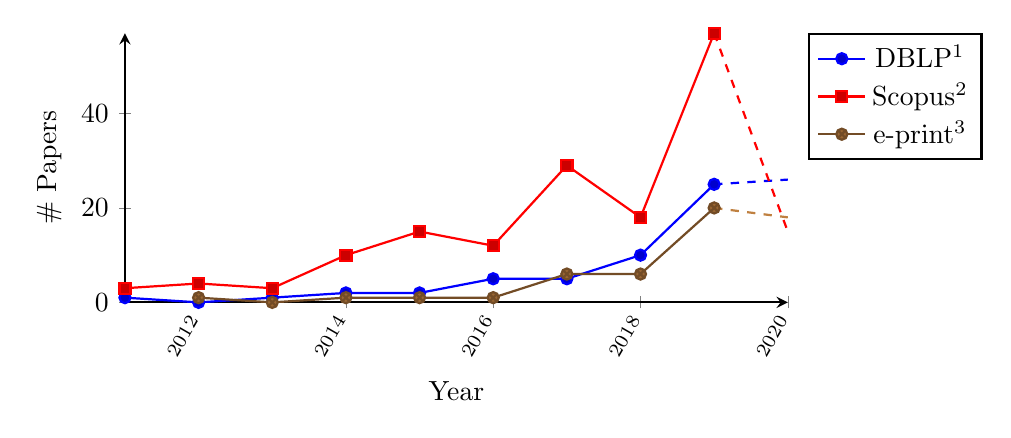
\begin{tikzpicture}
		\begin{axis}[width=10cm, height=5cm, xlabel={Year},ylabel={\# Papers},
		axis x line=bottom, axis y line=left, thick, xticklabel style=
{/pgf/number format/1000 sep=,rotate=60,anchor=east,font=\scriptsize},legend pos=outer north east]
			\addlegendentry{DBLP\footnotemark{}}
			\addplot coordinates {(2011, 1) (2012, 0) (2013, 1) (2014, 2) (2015, 2) (2016, 5) (2017, 5) (2018, 10) (2019, 25)};

			\addlegendentry{Scopus\footnotemark{}}
			\addplot coordinates {(2011, 3) (2012, 4) (2013, 3) (2014, 10) (2015, 15) (2016, 12) (2017, 29) (2018, 18) (2019, 57)};

			\addlegendentry{e-print\footnotemark{}}
			\addplot coordinates {(2012, 1) (2013, 0) (2014, 1) (2015, 1) (2016, 1) (2017, 6) (2018, 6) (2019, 20)};

			\addplot[blue, dashed] coordinates {(2019, 25) (2020, 26)};
			\addplot[red, dashed] coordinates {(2019, 57) (2020, 15)};
			\addplot[brown, dashed] coordinates {(2019, 20) (2020, 18)};
		\end{axis}
	\end{tikzpicture}
	\caption{Queries to scientific databases, by August 31, 2020.}
	\label{fig:growing_interest}
\end{figure}


\subsection{The Drawbacks of Deep Learning in Side-Channel Analysis}
\label{sec:drawbacks_dl}
The successful breakthrough of the \gls{dl} approach in many application fields gave the opportunity to their respective specialists to draw comparisons with former state-of-the-art \gls{ml} algorithms.
Most of the time, the same criticism emerged from those comparisons: \gls{dl} appeared as alchemy.
Indeed, some intriguing results emphasized that \glspl{dnn} are more prone to \emph{over-fitting}, a phenomenon where the learning algorithm starts to learn \emph{by heart} in order to improve its performances, although this strategy generalizes poorly for most of the investigated learning problems.
Likewise, research has shown that machine learning algorithms could be fooled by a malicious person, thus questioning the reliability of such algorithms in a security context.
This line of works, entitled \glspl{gan} has recently skyrocketed in the \gls{dl} literature with impressive results~\cite{goodfellow_generative_2014}.

Those drawbacks have legitimately found some echoes in the \gls{sca} community, where only realizing and assessing an attack is not sufficient to draw exhaustive conclusions for a security evaluation.
Therefore, one may question the interest of such an approach in a security evaluation.
In particular, the different attack methodologies proposed so far in the literature could be easily interpretable by simple statistical tools, which is not the case of \gls{dl}-based algorithms which are often seen as black-boxes, so it is hard for the \gls{sca} practitioner to interpret and to rely on such results.
Moreover, the fact that \gls{dl} algorithms can be fooled does help to bring trust in a community whose work is especially grounded on trust.
It is noticeable yet that the scenarios where the \gls{dl} algorithms are fooled assume that the latter ones are the target themselves and that the malicious entity have access to some inputs/outputs of the algorithm.
Actually, this is the convert situation of ours, in which this is the attacker who is equipped with \gls{dl} methods, and not the target.
Still, this confusion may lead the layman attacker to have misconceptions about the strengths and the weaknesses of \gls{dl} for \gls{sca}.

\addtocounter{footnote}{-2} %3=n
\footnotetext{\url{https://dblp.uni-trier.de/search?q=side\%20channel\%20learning}}
\addtocounter{footnote}{1} %3=n
\footnotetext{Query ``TITLE-ABS-KEY(("learning") AND ("SCA" OR "side-channel") AND ("attacks") AND ("cryptographic" OR "cryptography" OR "crypto"))  '' on \url{www.scopus.com}}
\addtocounter{footnote}{1} %3=n
\footnotetext{Query ``learning side channel'' at \url{eprint.iacr.org}, excluding the \gls{lwe}-related keywords}